\documentclass{IEEEcsmag}

\usepackage[colorlinks,urlcolor=blue,linkcolor=blue,citecolor=blue]{hyperref}

\usepackage{upmath}
\usepackage{amssymb}
\usepackage{amsmath}
\usepackage{array}
\newcolumntype{P}[1]{>{\centering\arraybackslash}p{#1}}

\jvol{XX}
\jnum{XX}
\paper{8}
\jmonth{May/June}
\jname{Computing in Science and Engineering}
\pubyear{2021}
\newtheorem{theorem}{Theorem}
\newtheorem{lemma}{Lemma}

\setcounter{secnumdepth}{0}

\begin{document}

\sptitle{Department: Head}
\editor{Editor: Name, xxxx@email}

\title{PyExaFMM: Designing a high-performance particle fast multipole solver in Python with Numba}

\author{S. Kailasa}
\affil{Department of Mathematics, University College London}

\author{T. Betcke}
\affil{Department of Mathematics, University College London}

\author{T. Wang}
\affil{Department of Mechanical and Aerospace Engineering, The George Washington University}

\author{\text{L}. A. Barba}
\affil{Department of Mechanical and Aerospace Engineering, The George Washington University}

\markboth{Department Head}{Paper title}

\begin{abstract}
The particle fast multipole method [FMM] is a good case study for understanding the efficacy of Python for developing high-performance software for non-trivial algorithms, due its reliance on a hierarchical tree data structure. In this paper we explore the mathematical and software design techniques used to extract performance for PyExaFMM, a Python based FMM solver accelerated with Numba, designed to be run on single-node multicore architectures. We report that we achieve runtimes within $\mathcal{O}(N)$ of the state of the art C++ implementation, with comparable accuracy and memory footprint for three dimensional problems in double precision.
\end{abstract}

\maketitle
\chapterinitial{We introduce PyExaFMM}\footnote{https://www.github.com/exafmm/pyexafmm}

- What's the context of PyExaFMM?
	- Compiled language implementations exist
	- Numba JIT compiler for Python can translate hot loops code to efficient machine code.
	- Python is well understood in SC community.
	- FMM is a benchmark for complex SC software built using Python alone.
- This paper consists of:
	- Brief intro to FMM algorithm (<1000 words)
	- Math methods, software design and parallelization strategies for achieving performance with Numba. (~2500 words)
	- Benchmarks wrt comparable C++ module (~1500 words)

\section{FAST MULTIPOLE METHODS}


% Larger figure
\begin{figure*}
	\centerline{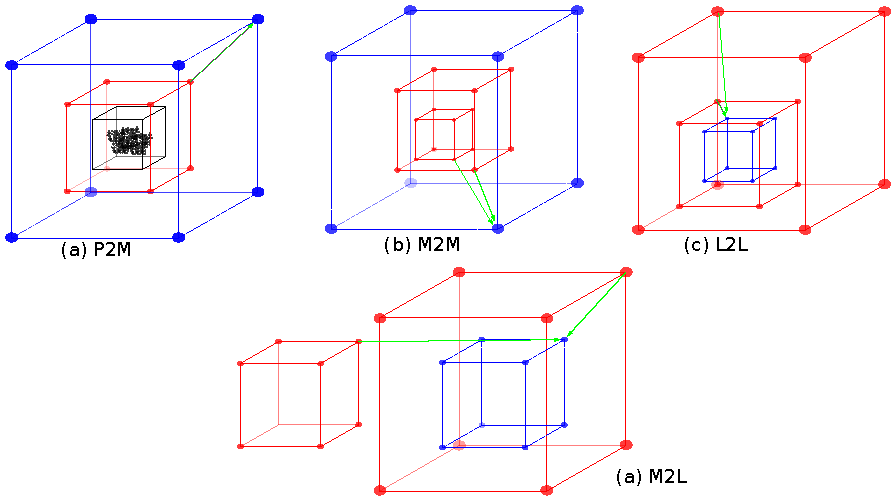
\includegraphics {figures/operators.pdf}}
	\caption{The operators of the KIFMM. Equivalent surfaces are shown in red, check surfaces in blue, and the charged points in black. Surfaces are plotted with 8 quadrature points, one at each vertex.}
	\label{fig:operators}
\end{figure*}


\section{HIGH PERFORMANCE PYTHON WITH NUMBA}


\section{TECHNIQUES FOR ACHIEVING PERFORMANCE}


\subsection{Efficient Operators}

% \begin{table*}
% 	\centering
% 	\caption{Relative error, runtime and peak memory consumption in comparison to the SOTA. Experiments run with $N=1,000,000$ points tested in two geometries: (1) distributed randomly in a cubic unit box, (2) distributed randomly on the surface of a sphere with unit radius, leading to $M$ leaves in their respective geometries, with a maximum of $150$ points per leaf, multipole and local expansions of order $p$, and a compression rank $k=50$ for PyExaFMM. Charge densities are chosen in the interval $[0, 1)$. Runtimes are calculated 7 times for statistics and reported to 1 significant figure with respect to their standard deviation, and exclude tree building time. Error and peak memory consumption are reported to 3 significant figures after one run.}
% 	\begin{tabular}{|*{10}{c|}}
% 		\hline
% 		& & &   & \multicolumn{2}{c|}{Runtime} & \multicolumn{2}{c|}{Peak Memory} & \multicolumn{2}{c|}{Relative Error}\\
% 		\hline
% 		$N$ & $M$ &$p$ &  Geometry   &   PyExaFMM  &  ExaFMM-T &    PyExaFMM  &  ExaFMM-T  &   PyExaFMM  &  ExaFMM-T\\
% 		\hline
% 		1,000,000 & 17,017 & 4   &   Sphere  &  $10.6 \pm 0.1$ s & $0.41 \pm 0.04$ s  &  2.96 GB  &   2.34 GB  & 1.00e-4 & 8.75e-5\\
% 		 & 32,768 &    &   Random  &  $13.2 \pm 0.2$ s &  $0.41 \pm 0.05$ s &  4.93 GB  &   2.98 GB  & 8.75e-5 & 7.66e-5\\
% 		&  & 5   &   Sphere  &    $33.8 \pm 0.8$ s & $1.28 \pm 0.03$ s &  3.00 GB  &  2.53 GB  & 4.55e-6 & 4.15e-6\\
% 		 &  &   &   Random  &  $65 \pm 2$ s &    $1.46 \pm 0.04$ s  &  4.93 GB  &   3.32 GB  & 2.81e-6 & 3.91e-6\\
% 		 &  & 6   &   Sphere  &  $41.0 \pm 0.7$ s &   $1.48 \pm 0.01$ s  &  3.04 GB  &   2.80 GB  & 2.41e-6 & 1.67e-6\\
% 		 &  &    &   Random  &  $71 \pm 4$ s &   $1.66 \pm 0.04$ s  &  4.93 GB  &   3.55 GB  & 1.59e-6 & 3.41e-6\\
% 		 &  & 7   &   Sphere  &  $57.0 \pm 0.1$ s &  $1.78 \pm 0.04$ s  &  3.09 GB  &   3.22 GB  & 2.00e-6 & 2.86e-6\\
% 		 &  &    &   Random  & $131 \pm 2$ s &   $2.11 \pm 0.06$ s  &  4.93 GB  &   3.88 GB  & 1.71e-6 & 3.84e-6\\
% 		\hline
% 	\end{tabular}
% 	\label{tab:performance}
%  \end{table*}

% Larger figure
% \begin{figure*}
% 	\centerline{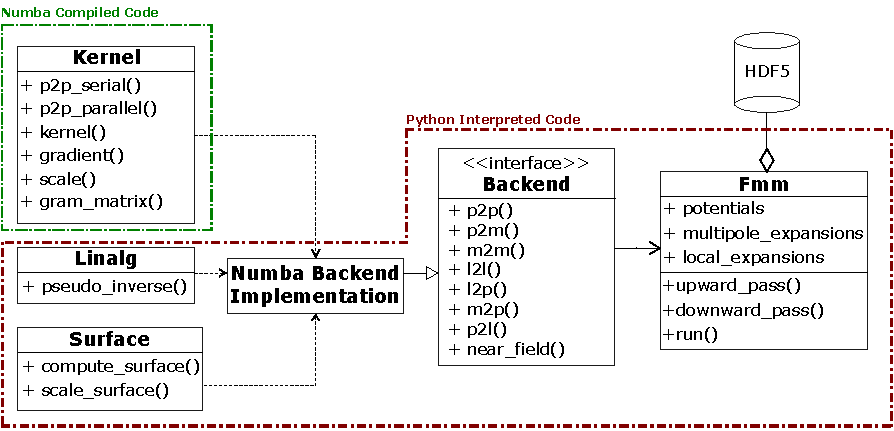
\includegraphics {figures/software.pdf}}
% 	\caption{Simplified UML model of all PyExaFMM components. Trees and operators are precomputed and stored in the HDF5 database. Except for the `Fmm' object which acts as the user interface, all other components are modules consisting of simple functions.}
% 	\label{fig:design}
% \end{figure*}

% \begin{table}
% 	\centering
% 	\caption{Effect of compression rank $k$, with multipole and local expansions of order $p=5$, corresponding to $n=98$ quadrature points, for FMM problem with 100,000 randomly distributed points, and a maximum of 150 points per leaf. Point coordinates and charge densities are chosen in the interval [0, 1). Runtimes calculated seven times for statistics, peak memory consumption and relative error reported to 3 significant figures after one run.}
% 	\begin{tabular}{ |P{10pt}|P{45pt}|P{47pt}|P{47pt}|}
% 		\hline
% 		$k$ & Runtime & Peak Memory & Relative Error\\
% 		\hline
% 		10 & $6.89 \pm 0.11$s &   663 MB & 1.51e-4\\
% 		20 & $6.89 \pm 0. 09$s &  667 MB & 2.24e-5\\
% 		30 &  $6.93 \pm 0. 11$s&  672 MB & 1.15e-5\\
% 		40 &  $6.95 \pm 0. 09$s &  676 MB & 3.67e-6\\
% 		98 &  $15.44 \pm 0. 55$s &  685 MB & 2.43e-6\\
% 		\hline
% 	\end{tabular}
% 	\label{tab:compression}
%  \end{table}

\section{PERFORMANCE}


\section{CONCLUSION}


\section{ACKNOWLEDGMENT}

SK is supported by EPSRC Studentship 2417009.

\bibliography{pyexafmm}
\bibliographystyle{ieeetr}

\begin{IEEEbiography}{Srinath Kailasa}{\,}is a Graduate Student at University College London, currently pursuing a PhD in Computational Mathematics. He received an MPhys in Physics (2017) and an MSc in Scientific Computing (2020) from the University of Durham, and University College London respectively, interspersed with time as a Software Engineer in industry. His research interests are in high-performance and scientific computing. Contact him at srinath.kailasa.18@ucl.ac.uk.
\end{IEEEbiography}

\begin{IEEEbiography}{Timo Betcke}{\,}is Professor of Computational Mathematics at University College London. Is the lead investigator of the Bempp project, an open-source boundary element library. He studied Engineering in Germany as Undergraduate and then completed a PhD in Oxford in Numerical Analysis. From 2005 to 2006 he had various research positions until he became a Lecturer at UCL in 2011. Since 2018 he is a full Professor in the Department of Mathematics at UCL. Contact him at t.betcke@ucl.ac.uk.
\end{IEEEbiography}

\begin{IEEEbiography}{Tingyu Wang}{\,}is a PhD student in Mechanical Engineering at the George Washington University. Contact him at twang66@email.gwu.edu.
\end{IEEEbiography}

\begin{IEEEbiography}{Lorena. A. Barba}{\,}is a Professor of Mechanical and Aerospace Engineering at the George Washington University.  Contact her at labarba@email.gwu.edu.
\end{IEEEbiography}

\end{document}

